\documentclass[xcolor=table]{beamer}
\usepackage{etex}
\usepackage{pgfpages}
\usepackage[utf8]{inputenc}
\usepackage[spanish]{babel}
\usepackage{caption}
\usepackage{subcaption}
\usepackage{pgfplots}
\usepackage{tikz}
\usepackage{tkz-kiviat}
\usepackage{fixpauseincludegraphics}
\usepackage{booktabs}
\usepackage{filecontents}
\usepackage{rotating}


\usetikzlibrary{shapes,arrows}
%
%% Buscar más en http://deic.uab.es/~iblanes/beamer_gallery/individual/Malmoe-dolphin-default.html
\usetheme{Malmoe}
%%\usecolortheme{dolphin}
\usecolortheme{lily}
\setbeamercovered{transparent}
\setbeamercolor{block title}{use=structure,fg=white,bg=blue!75!white}
\setbeamercolor{block body}{use=structure,fg=black,bg=gray!20!white}
\newcommand{\cs}{%
  {\settoheight{\dimen0}{C}C\kern-.05em \resizebox{!}{\dimen0}{\raisebox{\depth}{\fontseries{b}\selectfont\#}}}}
%
%
%\setbeameroption{show notes on second screen} % Descomentar para no ver comentarios

% Esto agrega un número romano a los siguientes, para romper un frame en dos
% utilizar
%       \framebreak{}
\setbeamertemplate{frametitle continuation}[from second][(\insertcontinuationcountroman)]

\AtBeginSection[]
{
  \begin{frame}
    \frametitle{Índice}
    \tableofcontents[currentsection]
  \end{frame}
}


%%%%%%%%%%%%%%%%%%%%%
% Datos de la tesis %
%%%%%%%%%%%%%%%%%%%%%

\author[Mirta González y Arturo Volpe]{Mirta González \quad Arturo Volpe}

\title[Juegos serios como apoyo a la enseñanza
tradicional\hspace{2em}\insertframenumber/\inserttotalframenumber]%
{Juegos serios como apoyo a la enseñanza tradicional:  una aplicación a la
    formación de profesionales del área de enfermería}

%\date{Mayo, 2014} %leave out for today's date to be insterted

\institute{Universidad Nacional de Asunción\\Facultad Politécnica}

\begin{document}


%\end{frame}

\frame{\titlepage}

\begin{frame}
\frametitle{Índice}
\tableofcontents
\end{frame}

\section{Introducción}
\setcounter{sectiontotal}{3}

\begin{frame}
\frametitle{\pagetitle}
\framesubtitle{Descripción}
\begin{figure}
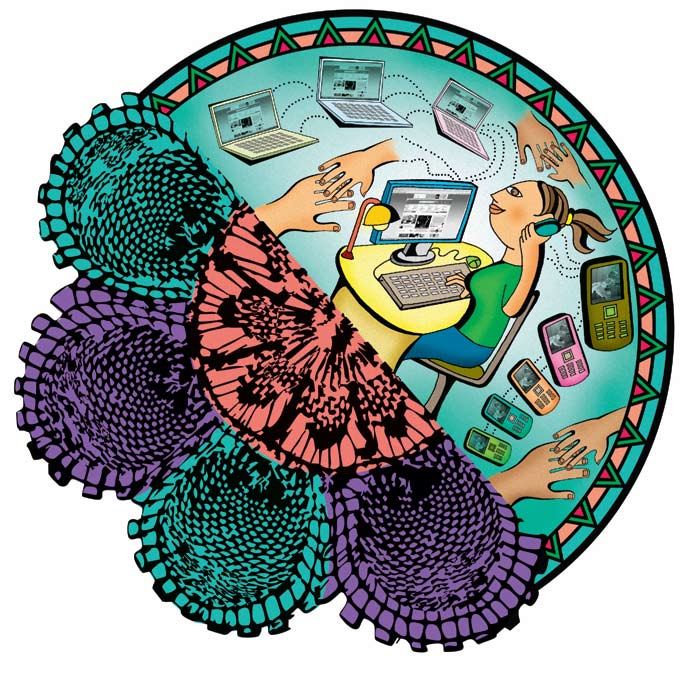
\includegraphics[scale=.3]{imagenes/nhanduti}
\end{figure}
\end{frame}

\begin{frame}
\frametitle{\pagetitle}
\framesubtitle{Objetivo general}
\begin{block}{Descripción}
\centering
Identificar y valorar los aspectos pedagógicos, de diseño, de implementación y
de evaluación que influyen a la creación de herramientas educativas que utilizan
las corrientes pedagógicas actuales apoyadas en las TIC, especialmente los
juegos serios.
\end{block}


\end{frame}

\begin{frame}
\frametitle{\pagetitle}
\framesubtitle{Objetivos específicos}

\small
\begin{itemize}[<+->]
\item Proveer una visión actualizada de las corrientes pedagógicas apoyadas con las TIC.
\item Proveer una visión actualizada de los juegos serios.
\item Identificar áreas de aplicación de los juegos serios.
\item Seleccionar las herramientas tecnológicas disponibles para el desarrollo de juegos serios.
\item Contrastar en la práctica los conocimientos teóricos adquiridos a través del diseño
e implementación de un juego serio.
\item Evaluar la solución propuesta para identificar los
aspectos de diseño, desarrollo y evaluación de los juegos serios.
\end{itemize}
\end{frame}


\section{\Gls{tic} en la educación}
%1/2 página

Las \Gls{tic} son un conjunto de herramientas tecnológicas y recursos utilizados para
comunicar, crear, diseminar, almacenar y manejar la
información\cite{unesco:ict}. Estas tecnologías abarcan computadoras
personales,internet, radio, televisión y telefonía\cite{tinio:ict} entre otros.

La utilización actual de las \Gls{tic} en la educación no es un fenómeno aislado,
responde a una evolución constante de la tecnología y metodología utilizada.
Existen cuatro pedagogías de entre varias en las que las tics han sido
utilizadas de manera activa, las cuales son el instruccionismo o educación
tradicional, el conductismo, el constructivismo y finalmente, el
construccionismo. Esto no implica que las tics no puedan ser aplicadas a otras
pedagogías, es más, existen otras corrientes que utilizan las \Gls{tic}, de diversas
maneras como el cognoscitivismo\cite{egenfeldt2007third} y el
conectivismo\cite{white:ict}. 

Este trabajo se basa en el construccionismo, pedagogía según la cual el
conocimiento es construido por el estudiante en lugar de ser trasmitido por el
profesor\cite{moses:2003} y esto sucede particularmente cuando el mismo se
involucre en la elaboración de un producto o artefacto que tenga un significado
y pueda ser compartido\cite{valdivia:sg}. El construccionismo y las tics siempre
han estado relacionados, ya que el mismo se originó con un lenguaje de
programación (LOGO)\cite{ict:ttc}. Posee un enfoque diferente en cuanto al uso
de las tics en la educación. Esta pedagogía se diferencia de la educación
tradicional en que el estudiante ya no es un receptor pasivo de información, en
cambio, el mismo participa activamente del proceso de aprendizaje construyendo
su propio conocimiento. Se diferencia del instruccionismo en que el
construccionismo utiliza la tecnología como medio cognitivo y no para la entrega
de contenido.

%\begin{itemize}
%\item Que son
%\item Educacion tradicional y mencionar las otras corrientes
%\item Construccionismo
%\end{itemize}
\section{Serious Game}
\label{sec:tics_JUEGO_SERIO}

Un \emph{Serious Game} es un vídeo juego elaborado con el propósito primario que
no es el de entretener\cite{sg:aoverview}, sino tienen una finalidad educativa
explícita y cuidadosamente pensada, utiliza la tecnología y los conceptos de la
industria de los vídeo juegos para encontrar solución a problemas reales. Es
decir, se utilizan para definir los juegos que poseen una pedagogía incluida,
algún tipo de evaluación ya sea interna o externa y lo que hay que aprender
(contenido) integrado\cite{damien:sg}.

Los \emph{Serious Game} proveen una oportunidad muy importante para ayudar en la
enseñanza y desarrollo de profesionales, por que ayudan a crear el tipo de
educación que los adultos prefieren, proveen mecanismos para que los estudiantes
cometan errores y experimenten con sus ideas, con su conocimiento y con la
teoría en un ambiente protegido sin riesgos para la vida o la identidad. 

Los beneficios que brindan los \emph{Serious Game} se acentúan en la medida en
la que los mismos proveen entornos más completos en donde realmente se puedan
poner en práctica la teoría, esto ayuda a una comprensión más profunda del área
de interés.

La principal diferencia entre los \emph{Serious Game} y otras aplicaciones de
\emph{E-Learing} es su enfoque en la creación de una experiencia de aprendizaje
significativo, relevante y atractivo. En un \emph{Serious Game} existen metas
claras de aprendizaje pero las mismas se encuentran en un contexto significativo
en donde se deben aplicar los conocimientos y hacer uso de herramientas que
están a disposición para obtener éxito en la resolución de los problemas
presentados. Estos problemas se equilibran a través de la retroalimentación y
otras estrategias para mantener el interés del estudiante
\cite{papertian:const}.
%. Todo esto hace que en los \emph{Serious Game} el principal objetivo sea ganar
%el juego no aprender, sin embargo sólo se puede hacer esto dominando el
%aprendizaje

\fixme{El campo de los \emph{Serious Game} rechaza la idea de que los profesionales de
    la educación pueden ser reemplazados fácilmente}{Obs: que es cada sección?,
    un enfoque? Una técnica? Un buzzword?}, para ellos la labor de estos
profesionales es imprescindible para la reflexión y orientación del aprendizaje.
Es cierto que se puede llegar a aprender sin el apoyo de un profesional de la
educación pero se corre el riesgo de perder el enfoque y la eficacia
\cite{elearning:seiousgames}. 

El \emph{serious Game} no se trata de una modelo de aprendizaje pasajero. Varios
autores como \emph{Johan Huizinga}, \emph{Jean Piaget}, \emph{Wittgenstin} y
\emph{Seymour Papert} han reconocido su importancia  como objeto de aprendizaje.
Los juegos deben ser elaborados teniendo en cuenta el nivel cognitivo del
estudiante, es decir, su etapa de aprendizaje y en que el aprendizaje difiere de
acuerdo a la etapa de vida en la que se encuentre un estudiante. Mediante la
práctica repetida de actividades relacionadas al área de interés se desarrollan
habilidades y destrezas\cite{education:games}. 

\observacion{Se podría hacer una comparación? (entre todos)}

Los siguientes son ejemplos de algunas áreas que utilizan Serious Game:

\begin{description}

\item[Militar] Los primeros juegos a menudo se basaban en lucha o combate.
	Durante más de 30 años los juegos han sido reconocidos como herramientas
	factibles en el entrenamiento de militares. En 1996 fue lanzado un juego
	llamado \emph{Marine Doom} en donde la tarea de los jugadores era el
	aprendizaje de formas de ataque, conservación de municiones, comunicarse
	con eficacia, dar órdenes al equipo de trabajo entre otros. De esta
	manera tuvo lugar una forma de entrenamiento más atractivo, sin el
	costo, dificultad, riesgos e inconvenientes que implicaría el mismo
	entrenamiento en un entorno real. Además se podían crear situaciones que
	en el mundo real serían muy difíciles de replicar y donde los errores
	pueden ser catastróficos además, permite la repetición hasta alcanzar la
	maestría\cite{education:games}.


\item[Salud] Este tipo de juegos son cada vez mayores, los juegos de salud se
	utilizan para la formación de profesionales basada en la simulación. En
	2008 el Centro de Simulación Hollier en Birmingham, Reino Unido, realizó
	una prueba que permitió a médicos jóvenes experimentar y entrenar para
	diversos escenarios médicos a través de maniquíes virtuales como
	pacientes, de este modo el aprendizaje se da por la experiencia. En su
	disertación, Roger D. Smith, realizó una comparación entre la enseñanza
	tradicional y la formación mediante realidad virtual y el uso de
	herramientas basadas en la tecnología de juegos en cuanto a la cirugía
	laparoscópica. Como conclusión afirmó que lo último era más barato,
	requería menos tiempo y que permitió menos errores médicos cuando los
	médicos se presentaban en una cirugía real debido a, entre otras cosas,
	la posibilidad de repetición de la experiencia sin riesgo
	alguno\cite{education:games}.



\item[Juegos corporativos] Este tipo de juegos se han utilizado para la
	selección de personal, la mejora de comunicación entre los directivos y
	su personal de confianza, y la formación de nuevos empleados. Un ejemplo
	de estos juegos es el INNOV8 de IBM que ayuda en el entrenamiento de los
	estudiantes acerca de la gestión de procesos de negocios. Los Serious
	Game pueden ser utilizados incluso para elaborar planes de
	negocios\cite{education:games}. 

\end{description}


\section{Planteamiento del problema}
\setcounter{sectiontotal}{8}

\begin{frame}{Estado actual del Instituto Andrés Barbero}

%\begin{figure}
%    \begin{subfigure}[b]{.6\linewidth}
%        \centering
%        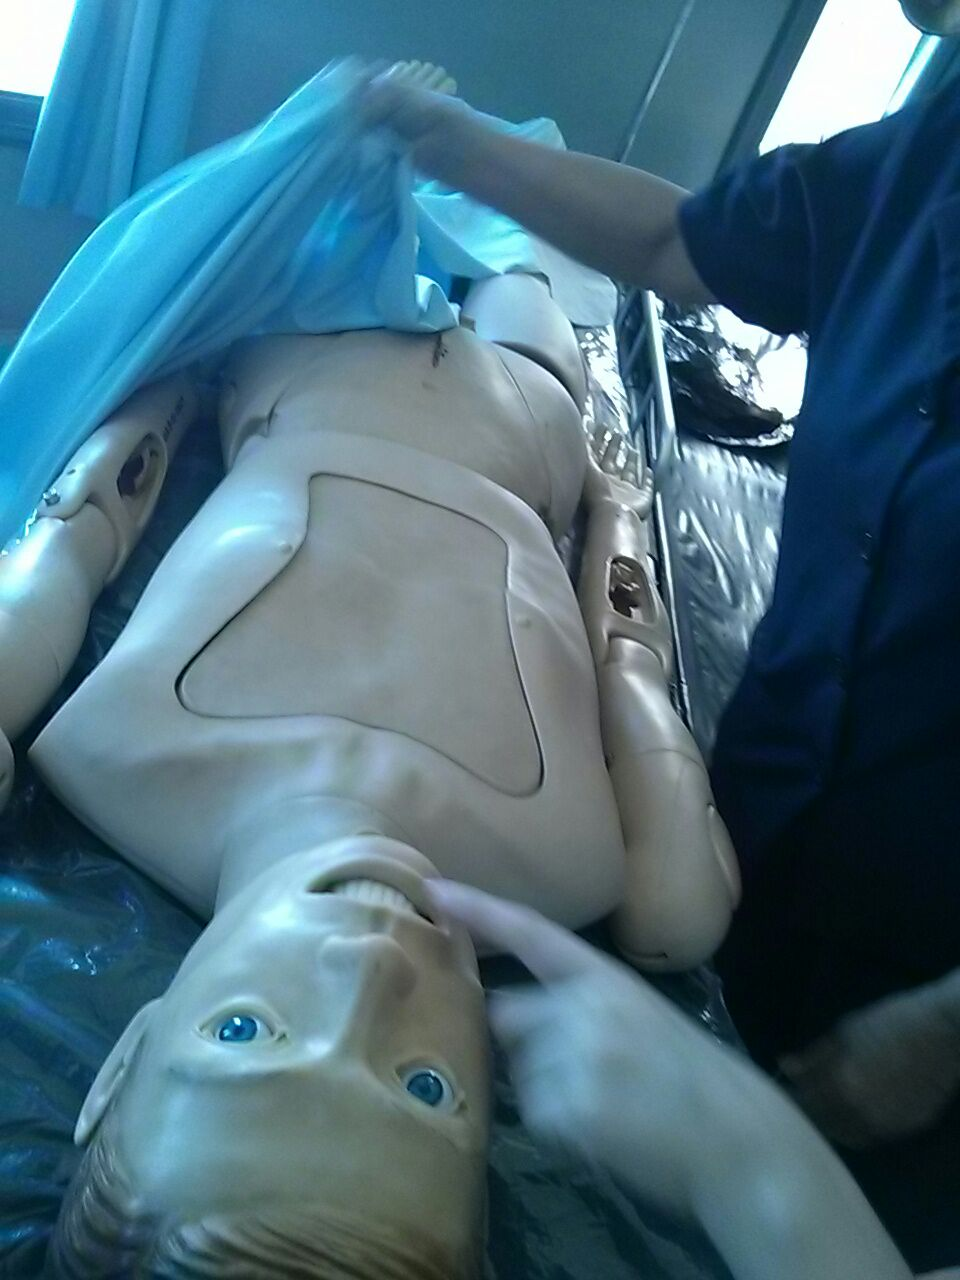
\includegraphics[height=3cm]{../problema/iab_sala_3.jpg}
%        \caption{Tiempo por tipo de actividad}
%    \end{subfigure}

    
%    \begin{subfigure}[b]{.6\linewidth}
	\begin{enumerate}[<+->]
	\item Prácticas en laboratorio
	\item Prácticas en hospitales o prácticas de campo
	\end{enumerate}
%	\end{subfigure}
%\end{figure}
\end{frame}

\begin{frame}{Problemas actuales del Instituto Andrés Barbero}
	\begin{enumerate}[<+->]
	\item Falta de preparación de los alumnos
	\item Definición de un protocolo de comunicación
	\item Nerviosismo ante la primera práctica
	\item Alta carga horaria de los trabajos prácticos
	\item Reducida carga horaria para el estudio de las materias teóricas
	\item Poca flexibilidad de los profesores
	\item Falta de materiales actualizados para los profesores
	\item Problemas de transporte
	\item Falta de preparación para las prácticas
	\item Alta cantidad de alumnos
	\end{enumerate}
\end{frame}

\begin{frame}{Propuesta de solución}
	\begin{enumerate}[<+->]
	\item Evaluación
	\item Progreso
	\item Tiempo de práctica
	\item Factor psicológico
	\item Ubicuidad
	\item Realismo
	\item Enfoque individual
	\end{enumerate}
\end{frame}

%\begin{frame}{Requerimientos de la solución}\end{frame}

\begin{frame}{Alcance de la solución (I)}
	Factores limitantes.
	\begin{enumerate}[<+->]
	\item Limitaciones técnicas
	\item Importancia de representación
	\item Facilidad de realización
	\end{enumerate}
\end{frame}

\begin{frame}{Alcance de la solución (II)}
	Hipótesis.
	\begin{enumerate}[<+->]
	\item Comando de voz con interfaz
	\item Extracción uniforme de elementos
	\item Acciones de bioseguridad
	\item Representación iconográfica
	\item Factores limitantes
	\item Falta de pistas
	\item Ubicuidad
	\end{enumerate}
\end{frame}

\begin{frame}{Alcance de la solución (III)}
	Decisiones de diseño.
	\begin{enumerate}[<+->]
	\item Acciones por interfaz de usuario
	\item Simulación integra de pasos
	\end{enumerate}
\end{frame}

\section{Tecnologías}

\begin{frame}{Requisitos técnicos}\end{frame}
\begin{frame}{Motor de videojuegos}
\begin{tabular}{\textwidth}{l|cccccccc}
\toprule
Característica / Motor &
Unreal Engine          &
CryEngine              &
ShiVa3D                &
Unity3D                &
Blender Game Engine \\
\midrule
Distribución & iOS, soporta otros dispositivos en la versión comercial. &
iOs, Android & iOS, Android, Windows Phone, BlackBerry & Android, WindowsPhone,
iOs, BlackBerry & Soporte en desarrollo para Android \\ 

Tienda de librerias & Sí, en estado Alpha & No, existen tiendas de
terceros & Sí & Sí & Sí \\

Tamaño de tienda & Mediana & Mediana & Pequeña & Grande & Grande \\

Comunidad & Grande & Moderada & Moderada & Grande & Grande \\
Licencia del entorno de desarrollo & Gratuita solo para uso no comercial &
Propietaria & Propietaria & Gratuita para uso no comercial & GPL \\

Formatos soportados & fbx, dds, raw, ASE & Formatos propios & dae & FBX, OBJ,
Max, Blend, dae, 3ds, dxf, MB, MA, etc & 3ds, dae, fbx, dxf, etc \\

Licencia del motor & Versiones antiguas gratuitas para uso no comercial.
& Gratuita solo para uso no comercial & Propietaria, solamente la versión Web es
gratis & Versión limitada gratis, disponible para uso no comercial & GPL \\

Curva de aprendizaje & Compleja & Compleja & Compleja & Sencilla & Compleja \\

Lenguajes de desarrollo & Unreal Script y C++ & C++, Lua & FlowGraph
(propietario) y Lua & \cs{}, UnityScript y Boo & Python y C++ \\

IDE & Si, propio & Sí, propio & Sí, propio & Sí, propio & Sí, propio \\
\bottomrule

\end{tabular}

\end{frame}
\begin{frame}{Otras tecnologías}\end{frame}
\begin{frame}{Otras tecnologías}\end{frame}


\section{Diseño e implementación}
\setcounter{sectiontotal}{1}
\pgfmathtruncatemacro\implpass{1}
\newcommand{\addstep}[2][0]{%
    \includegraphics<\implpass|handout:#1>[width=\textwidth]{#2}%
    \pgfmathtruncatemacro\implpass{\implpass+1}%

}

% TODO Agregar lo de los ECA!
% TODO mejorar esta imagen
\begin{frame}
\frametitle{\pagetitle}
\framesubtitle{Flujo de interacción}
\centering

\addstep{../solucion/images/pantalla_inicio.jpg} 
\addstep{imagenes/flujo/flujo2.png} 
\addstep{../solucion/images/hemocultivo_principal.jpg} 
\addstep{imagenes/flujo/flujo3.png} 
\addstep{../solucion/images/hemocultivo_gui.jpg} 
\addstep{imagenes/flujo/flujo4.png} 
\addstep{../solucion/images/hemocultivo_jeringa_ampliada.jpg} 
\addstep{imagenes/flujo/flujo6.png} 
\addstep{../solucion/images/resultado_hemocultivo.jpg}
\addstep{imagenes/flujo/flujo18.png} 
\addstep{imagenes/flujo/flujo8.png} 
% Glasgow
\addstep{../solucion/images/pantalla_inicio.jpg} 
\addstep{imagenes/flujo/flujo9.png}
\addstep{imagenes/flujo/flujo10.png}
%\addstep{imagenes/flujo/flujo11.png}
\addstep{imagenes/flujo/flujo12.png}
\addstep{imagenes/flujo/flujo13.png}
\addstep{imagenes/flujo/flujo14.png}
\addstep{../solucion/images/glasgow_comandos_voz.jpg}
\addstep{../solucion/images/glasgow_diagnostico.jpg}
\addstep{imagenes/flujo/flujo16.png}
\addstep{../solucion/images/resultado_glasgow.jpg}
%\addstep{imagenes/flujo/flujo17.png}

\end{frame}

\section{Evaluación}
\setcounter{sectiontotal}{10}

\begin{frame}[fragile]
    \frametitle{Pruebas preliminares}

\begin{filecontents}{interfazuso.dat}
n   p       s
1	9.38	6.48
2   5.88	4.64
3   7.75	3.13
\end{filecontents}
\pgfplotstableread{interfazuso.dat}{\InterfazUso}

\begin{figure}
    \begin{subfigure}[b]{.5\linewidth}
        \centering
        \begin{tikzpicture}[scale=.45]
           \begin{axis}[ybar,%
              legend pos=outer north east,
              xmin=0,
              xmax=4,
              xtick=data,
              symbolic x coords={0,1,2,3,4},
              ymin=0,ymax=10,
              %ytick={0,2,4,6,8,10},
              xticklabels={Contextual,Interfaz,Herramienta},
              ylabel= Tiempo,
              xlabel= Tipo de acción,
              bar width=10pt,
              %enlarge x limits={abs=2},
                ]   
        \addplot[color=blue,ybar,fill=blue!75,area legend] table [x = {n}, y = {p}] {\InterfazUso};
        \addlegendentry{Primer}
        \addplot[color=red,ybar,fill=red!75,area legend] table [x = {n}, y = {s}]
        {\InterfazUso};
        \addlegendentry[align=left]{Promedio \\ siguientes}
        \end{axis}
        \end{tikzpicture}
        \caption{Tiempo por tipo de actividad}
    \end{subfigure}\hfill
    \pause
    \begin{subtable}[b]{.5\linewidth}
        \scriptsize
        \centering
        \begin{tabular}{lr}
        \toprule
        Métrica & Disconformidad \\
        \midrule
        Calidad Gráfica         & {\color{green!90!black} 0.17} \\
        Interacción Entorno     & {\color{red!90}   0.50} \\
        Interacción Objetos     & {\color{red!90}   0.49} \\
        Características Entorno & {\color{green!90!black} 0.33} \\
        Usabililidad Interfaz   & {\color{red!90}   0.51} \\
        Integración Hardware    & {\color{green!90!black} 0.27} \\
        \bottomrule
        \end{tabular}
        \caption{Disconformidad por métrica}
    \end{subtable}
\end{figure}

\end{frame}

\begin{frame}{Encuesta para determinar muestra}

\begin{figure}
    \begin{subfigure}[b]{.3\linewidth}
        \centering
        \begin{tikzpicture}[thick,scale=0.35, every node/.style={transform shape}]
            \pie[
                %explode=.2,
                text=legend,
                %style=drop shadow,
                %radius=3,
                %scale font,
                explode={0.1,0.1,0.3,0.3}
                ]%
            {%
                31.2 / Plan pos-pago,
                57   / Paquetes pre-pago,
                5.4  / Sin acceso,
                6.4  / Acceso ocasional}
        \end{tikzpicture}
        \caption{Acceso a internet}
    \end{subfigure}\hfill
    \pause{}
    \begin{subfigure}[b]{.3\linewidth}
        \centering
        \begin{tikzpicture}[thick,scale=0.35, every node/.style={transform shape}]
            \pie[
                text=legend,
                rotate=61.3,
                explode={.1,.2,.2,.2}
                ]%
            {%
            61.3 / Android,
             8.6 / Symbian,
            12.9 / Windows Phone,
            17.2 / Otros}
        \end{tikzpicture}
        \caption{Sistema operativo}
    \end{subfigure}\\
    \pause{}
    \begin{subfigure}[b]{.5\linewidth}
        \centering
        \begin{tikzpicture}[thick,scale=0.35, every node/.style={transform shape}]
            \pie[
                text=legend,
                explode=.1
                ]%
            {%
                81.7 / Cumple,
                18.3 /  No Cumple
            }
        \end{tikzpicture}
        \caption{Cumplimiento de requisitos}
    \end{subfigure}
\end{figure}

\end{frame}

\begin{frame}[t,fragile]
\frametitle{Encuesta para evaluar conocimiento}
\centering

% Datos
\begin{filecontents}{objetiva.dat}
n	total        muestra	    control
1	0.2020159639 0.3636363636	0.1818181818
2	0.6027491017 0.6363636364	0.6
3	0.1332966457 0.09090909091	0.1363636364
4	0.2580191298 0.2727272727	0.2545454545
5	0.5869865976 0.8181818182	0.5636363636
6	0.1640933841 0	            0.1834862385
7	0.5256475617 0.6363636364	0.5137614679
8	0.2947317706 0.4545454545	0.2752293578
9	0.3081905611 0.1818181818	0.3211009174
10	0.4498120076 0.3636363636	0.4587155963
\end{filecontents}
\pgfplotstableread{objetiva.dat}{\Objetiva}

\begin{tikzpicture}[thick,scale=0.8, every node/.style={transform shape}]
\begin{axis}[
    title={},
    xlabel={Pregunta},
    ylabel={Puntos},
    xmin=1, xmax=10,
    ymin=0, ymax=1,
    xtick={0,1,2,3,4,5,6,7,8,9,10},
    ytick={0,.25,.50,.75,1},
    legend pos=outer north east,
    ymajorgrids=true,
    xmajorgrids=true,
    grid style=dashed,
]
 
\only<1->{\addplot[color=blue,] table [x = {n}, y = {muestra}] {\Objetiva};
\addlegendentry{Muestra}}
\only<2->{\addplot[color=red,] table [x = {n}, y = {control}] {\Objetiva};
\addlegendentry{Control}}
\only<3->{\addplot[color=black,dashed] table [x = {n}, y = {total}] {\Objetiva};
\addlegendentry{Total}}
 
\end{axis}
\end{tikzpicture}

\end{frame}
\begin{frame}{Comparación de rendimiento}

\begin{table}
\begin{tabular}{lr}
\toprule
Promedio usuarios & \textbf{3.82} \\
\onslide+<2->{Promedio control  & \textbf{3.47} \\\midrule}
\onslide+<3->{Promedio total    & \textbf{3.49}}
\\\bottomrule
\end{tabular}
\caption{Puntaje promedio por grupo}
\end{table}
\note{Estos datos no son estadísticamente válidos}
\note{El Incremento es del $10\%$}

\end{frame}

\begin{frame}{Apreciación de la solución}

\begin{figure}
    \scriptsize
    \centering
    \begin{subtable}[b]{.5\linewidth}
        \tiny
        \begin{tabular}{lc}
        \toprule
        Factores                 & Promedio encuesta \\
        \midrule
        Motivación               & De acuerdo \\
        Facilidad de exploración & De acuerdo \\
        Sensación de Inmersión   & De acuerdo \\
        Pedagogía                & De acuerdo \\
        Representación           & Parcialmente de acuerdo \\
        Retroalimentación        & Parcialmente de acuerdo \\
        Utilidad                 & De acuerdo \\
        \bottomrule
        \end{tabular}
        \caption{Aceptación por aspecto de la solución}
    \end{subtable}\hfill
    \pause
    \begin{subfigure}[b]{.5\linewidth}
        \tiny
        \begin{tikzpicture}[label distance=.15cm]
        \tkzKiviatDiagram[scale=.35,%
                            lattice=9,
                            %step=10,
                            ]
                        {Motivación,
                         Exploración,
                         Inmersión,
                         Pedagogía,
                         Representación,
                         Retroalimentación,
                         Utilidad}
        \tkzKiviatLine[thick,
                        color=blue!25!white,
                        mark=ball,
                        ball color=blue,
                        mark size=5pt,
                        opacity=.2, 
                        fill=blue!20](6.7,6.8,6.3,6.7,5.3,6.0,6.9)
        \tkzKiviatGrad[prefix={$0,$},unity=1](1) 
        \end{tikzpicture}
        \caption{Valores estandarizados}
    \end{subfigure}
\end{figure}

\end{frame}
\begin{frame}{Validación de hipótesis}


\begin{table}
\scriptsize
\centering
\begin{tabular}{lcr}
\toprule
& \multicolumn{2}{c}{Promedio} \\
%\cmidrule(c){2-3} 
\cmidrule(lr){2-3}
Hipótesis                        & Encuesta                & Estandarizado \\
\midrule
Comandos de voz con interfaz     & De acuerdo              & $0,55$ \\
Extracción uniforme de elementos & Parcialmente de acuerdo & $0,65$ \\
Acciones de bioseguridad         & De acuerdo              & $0,58$ \\
Representación iconográfica      & Parcialmente de acuerdo & $0,53$ \\
Factores motivadores             & De acuerdo              & $0,65$ \\
Falta de pistas                  & De acuerdo              & $0,61$ \\
\bottomrule
\end{tabular}
\caption{Aceptación por hipótesis}
\end{table}

\end{frame}

\begin{frame}{Utilización de la solución}

\begin{table}
\centering
\small
\begin{tabular}{lr}
\toprule
Partidas                         & 99 \\
Primera partida                  & 4 de Noviembre de 2014 \\
Última partida                   & 23 de Noviembre de 2014 \\
\midrule
\onslide+<2->{Tiempo total                     & 11.134 \\
Promedio de tiempo por partida   & 112}
\\\midrule
\onslide+<3->{Acciones                         & 2.944 \\
Promedio de acciones por partida & 30}
\\\midrule
\onslide+<4->{Usuarios                         & \textcolor{red}{8} \\
Promedio de partidas por usuario & 12}
\\\bottomrule
\end{tabular}
\caption{Utilización de la solución}
\end{table}

\end{frame}
\begin{frame}[t,fragile]
    \frametitle{Evolución \emph{Extracción de sangre}}

%Datos
\begin{filecontents}{registrohemocultivo.dat}
n   p   s
 1  11  14.3
 2  9   10.6
 4  3   3.3 
 5  3   6.8 
 6  3   5.8 
 7  4   4   
 9  16  0
10  3   7.2 
\end{filecontents}

\pgfplotstableread{registrohemocultivo.dat}{\RegHemocultivo}

\begin{figure}
\centering
\begin{tikzpicture}[scale=.7]
   \begin{axis}[ybar,%
      legend pos=outer north east,
      symbolic x coords={1,2,4,5,6,7,9,10},
      ymin=0,ymax=18,
      xtick=data,
      ytick={0,3,6,9,12,15,18},
      ylabel= Puntaje,
      xlabel= Alumno,
      bar width=6pt,
        ]   
\addplot[color=blue,ybar,fill=blue!75,area legend] table [x = {n}, y = {p}] {\RegHemocultivo};
\addlegendentry{Primer}
\addplot[color=red,ybar,fill=red!75,area legend] table [x = {n}, y = {s}] {\RegHemocultivo};
\addlegendentry[align=left]{Promedio \\ siguientes}
\end{axis}
\end{tikzpicture}
\caption{Evolución del puntaje en \emph{Extracción de sangre} por alumno}
\end{figure}

\end{frame}
\begin{frame}[t,fragile]
    \frametitle{Evolución \emph{Glasgow}}

%Datos
\begin{filecontents}{registroglasgow.dat}
n    p    s
1    1    1.5 
2    2    2.3 
4    1    1.5 
6    2    2 
7    0    1 
\end{filecontents}
\pgfplotstableread{registroglasgow.dat}{\RegGlasgow}

\begin{figure}
\centering
\begin{tikzpicture}[scale=.7]
   \begin{axis}[ybar,%
      legend pos=outer north east,
      symbolic x coords={1,2,4,6,7},
      ymin=0,ymax=4,
      xtick=data,
      ytick={0,1,2,3,4},
      ylabel= Puntaje,
      xlabel= Alumno,
        ]   
\addplot[color=blue,ybar,fill=blue!75,area legend] table [x = {n}, y = {p}] {\RegGlasgow};
\addlegendentry{Primer}
\addplot[color=red,ybar,fill=red!75,area legend] table [x = {n}, y = {s}] {\RegGlasgow};
\addlegendentry[align=left]{Promedio \\ siguientes}
\end{axis}
\end{tikzpicture}
\caption{Evolución del puntaje en \emph{Evaluación Glasgow} por alumno}
\end{figure}

\end{frame}

\begin{frame}{Correlación}

\begin{table}
\scriptsize
\centering
\begin{tabular}{lrc}
\toprule
Factores                                                    & Valor         & Interpretación \\
\midrule
\onslide+<1->{Tiempo de uso y puntaje máximo extracción     & \textbf{0.62} & Positiva Fuerte}\\
\onslide+<2->{Tiempo de uso y puntaje máximo glasgow        & \textbf{0.78} & Positiva Muy Fuerte}\\
\onslide+<3->{Puntaje máximo extracción y encuesta objetiva & \textbf{0.44} & Positiva Fuerte}\\\bottomrule
\end{tabular}
\end{table}

\end{frame}

\section{Conclusiones}
\setcounter{sectiontotal}{7}

% Estado del arte
\begin{frame}
\frametitle{\pagetitle}
\framesubtitle{Estado del arte}
\begin{itemize}[<+->]

% REVISAR
\item Beneficios no explotados de las TIC

%\item El construccionismo y el constructivismo son pedagogías útiles para el
%desarrollo de habilidades profesionales

\item Los juegos serios permiten una experiencia sin riesgos

%\item Los juegos serios actuales ofrecen una retroalimentación muy guiada

\item La enseñanza de enfermeros es un área propicia para la
aplicación de los juegos serios

\end{itemize}
\end{frame}

\begin{frame}
\frametitle{\pagetitle}
\framesubtitle{Contexto de aplicación}
\begin{itemize}[<+->]
\item En el IAB, los juegos serios poseen potencial para resolver los problemas de la formación de los profesionales de enfermería

\item Se debe brindar herramientas alternativas de bajo costo
\end{itemize}
\end{frame}

% Diseño del juego serio
\begin{frame}
\frametitle{\pagetitle}
\framesubtitle{Diseño}
\begin{itemize}[<+->]


\item La definición del contenido debe ser realizada con profesores de 
práctica y directores de carrera

\item La motivación se incrementa al utilizar puntaje por procedimientos

\item La exploración es facilitada por los estados aleatorios

\item La inmersión es aumentada con la utilización de gráficos 3D
y partidas cortas

\item Se debe proveer retroalimentación sobre el desempeño del usuario sólo
al finalizar la partida

%\item La información sobre el rendimiento del usuario debe ser detallada

%\item Se deben utilizar indicadores de realización de acciones

\item Limitar la manipulación del punto de vista al utilizar elementos

\end{itemize}
\end{frame}

% Implementación del juego serio
\begin{frame}
\frametitle{\pagetitle}
\framesubtitle{Implementación}
\begin{itemize}[<+->]

%\item El desarrollo de juegos serios difieren del desarrollo de software tradicional 
%en cuanto a la interacción y el uso de gráficos en tres dimensiones

%\item El uso de un motor de videojuego facilita el desarrollo

%\item Se recomienda tener en cuenta el costo, requisitos mínimos, familiaridad,
%    librerías, tienda y comunidad al seleccionar un motor de videojuego
    
%\item El uso de un motor de reglas condicionado por eventos es suficiente

\item Es necesario evaluar al usuario sin conexión a internet

\item Es costoso diseñar personajes y entornos en tres dimensiones
%\item Se deben diseñar personajes sólo cuando se requiere un alto nivel de
%    detalle o interacción

\item Es necesario enviar automáticamente los registros de utilización 

\end{itemize}
\end{frame}

\begin{frame}[noframenumbering]
\frametitle{\pagetitle}
\framesubtitle{Selección de tecnología}
\begin{itemize}[<+->]

\item Se recomienda utilizar Unity3D 

\item Se recomienda tener en cuenta el costo, requisitos mínimos, familiaridad,
librerías, tienda y comunidad al seleccionar un motor de videojuego

\item El uso de un motor de reglas condicionado por eventos es suficiente para
evaluar al usuario

\end{itemize}
\end{frame}

% Evaluación
\begin{frame}
\frametitle{\pagetitle}
\framesubtitle{Evaluación}
\begin{itemize}[<+->]

\item Validar relevancia y dificultad de temas a tratar en las pruebas de conocimiento 
con los profesores de cátedra

\item Es necesario poder reproducir las sesiones de juego del usuario con los
registros de uso

\end{itemize}
\end{frame}

% Ventajas y desventajas
\begin{frame}
\frametitle{\pagetitle}
\framesubtitle{Ventajas}
\begin{itemize}[<+->]

%\item La utilización de dispositivos móviles permite su uso en cualquier lugar y momento

\item Las soluciones basadas en dispositivos móviles son factibles de aplicación en el Paraguay

\item La solución es beneficiosa para el aprendizaje de procedimientos de enfermería según el $100\%$ de los alumnos que la evaluaron

%\item La solución agrega un nivel adicional de preparación entre las clases teóricas y la práctica con pacientes

\item Existe una recepción positiva ante la utilización de los juegos serios

%\item Los juegos serios ayudan a los estudiantes de enfermería a poner a prueba sus conocimientos

\end{itemize}
\end{frame}

\begin{frame}
\frametitle{\pagetitle}
\framesubtitle{Desventajas}
\begin{itemize}[<+->]

\item Alto costo de implementación

\item No existen generadores de contenido para juegos serios

%\item Los alumnos no cuentan con dispositivos móviles de altas prestaciones

%\item La principal dificultad para utilizar en mayor medida la solución es el factor tiempo según el $64\%$ de los alumnos que la evaluaron

\end{itemize}
\end{frame}

\section{Trabajos futuros}
\setcounter{sectiontotal}{1}

\begin{frame}{Trabajos Futuros}
    \begin{itemize}[<+->]
        \item Nuevos escenarios de práctica
        \item Visión de progreso
        \item Control del progreso por parte de los docentes
        \item Multijugador
        \item Éscenarios dinámicos
        \item Exploración de plataformas de realidad virtual
        \item Dificultad de acuerdo al alumno
    \end{itemize}
\end{frame}



\end{document}
